\chapter{Algoritmi}
In questo capitolo si analizzano a fondo i principali algoritmi di ordinamento e i relativi tempi di esecuzione. Nello specifico, si utilizzerà come modello di riferimento la macchina RAM con un criterio di costo costante, come analizzato nei capitoli precedenti. Prima di proseguire nella trattazione è necessario dare una definizione generale di algoritmo:

\begin{definition}
  Un algoritmo è una procedura di calcolo ben definita che prende un certo valore, o un insieme di valori, in input e genera un valore, o un insieme di valori, in output. Dunque, un algoritmo è una serie di passi computazionali che trasformano l'input in output.
\end{definition}

Un algoritmo può anche essere visto come uno strumento per la risoluzione di un problema computazionale ben definito: sotto questo sguardo, un algoritmo si definisce corretto se, per ogni istanza di input, termina con l'output corretto. Se un algoritmo è corretto, allora risolve quel determinato problema computazionale. Esistono molti modi per poter specificare un determinato algoritmo: si può utilizzare la lingua italiana o inglese, ma anche un linguaggio di programmazione come C, C++, JAVA e Pascal, o ancora tramite uno pseudocodice.

\section{Pseudocodifica}
La pseudocodifica può avvenire in molti modi, ma nel seguito si utilizzerano le convenzioni qui riportate:
\begin{itemize}
  \item L'indentazione serve ad indicare la struttura a blocchi dello pesudocodice, in modo da comprendere quali istruzioni appartengono, per esempio, ad un ciclo \code{for}, a un ciclo \code{while} o ad un \code{if}-\code{else} statement. Non sono utilizzate le parentesi graffe o parole chiave come begin ed end in quanto appesantiscono la sintassi;
  \item I costrutti iterativi \code{while}, \code{for}, \code{repeat-until} e il costrutto condizionale \code{if-else} hanno interpretazioni simili a quelle dei comuni linguaggi di programmazione. Il contatore del ciclo mantiene il suo valore dopo la fine del ciclo, quindi il valore che ha provocato la terminazione del ciclo stesso. Inoltre, si utilizza la parola chiave \code{to} quando il ciclo \code{for} incrementa il valore del suo contatore ad ogni iterazione, mentre si utilizza la parola chiave \code{down to} nel caso la variabile venga decrementata;
  \item Le assegnazioni di un valore ad una certa variabile avviene con il simbolo \code{:=}, differente dall'operatore \code{=}, che invece indica l'eguaglianza di due valori all'interno di un costrutto \code{if};
  \item Per identificare un elemento appartenente ad un array, si utilizza la notazione con le parentesi quadre, al cui interno si indica l'indice dell'elemento a cui si vuole accedere: \code{array[i]}; Per indicare un intervallo di valori all'interno dell'array si utilizza la seguente sintassi: \code{array[i..j]}, con cui si indica la sottomatrice composta dagli elementi compresi fra \(i\) e \(j\); 
  \item I dati utilizzati sono tipicamente organizzati in oggetti, formati da attributi, a cui si accede tramite la notazione punto: \code{oggetto.prop}. Le variabili che rappresentano un determinato oggetto sono trattate come puntatori a tale oggetto. Un puntatore che non fa riferimento ad alcun oggetto è inizializzato con il valore \code{NIL};
  \item I parametri vengono passati ad una procedura per valore: la procedura chiamata riceve una sua copia dei parametri e, quindi, se a una di queste variabili è assegnato un nuovo valore, la modifica non è visibile dalla procedura chiamante. Nel caso venga passato come argomento un oggetto, viene copiato il puntatore a tale oggetto e quindi le modifiche sono visibili anche dalla procedura chiamante;
  \item L'istruzione \code{return} restituisce immediatamente il controllo al punto in cui la procedura chiamante ha effettuato la chiamata. Le istruzioni \code{return} possono anche ritornare un valore al chiamante;
  \item Gli operatori booleani \code{and} e \code{or} sono cortocircuitati. Ciò significa che nella valutazione dell'espressione \code{x and y}, si valuta prima se il valore di \code{x} sia falso, in quanto, se lo fosse, l'intera espressione sarebbe falsa e non avrebbe quindi alcun senso valutare il valore della variabile \code{y}. Al contrario, nella valutazione dell'espressione \code{x or y}, si verifica innanzitutto se il valore di \code{x} sia vero, in quanto, se lo fosse, l'intera espressione sarebbe vera e non avrebbe quindi alcun senso valutare il valore della variabile \code{y}.
\end{itemize}

Tramite queste regole è possibile definire un generico algoritmo.

\section{Insertion Sort}
Una classe di algoritmi molto studiati è quella riguardante l'ordinamento di un vettore, che consiste nella disposizione dei suoi elementi in ordine crescente.

\vspace{10pt}

Il primo algoritmo analizzato è l'\textbf{insertion sort}, che prende in input una sequenza di \(n\) numeri \([a_1, a_2, ...,a_n]\) e restituisce in output una permutazione \([a_1', a_2',...,a_n']\) tale che \(a_1'\le a_2' \le ... \le a_n'\). Questo algoritmo ordina sul posto \footnote{L'algoritmo risistema gli elementi della sequenza all'interno dell'array avendo, in ogni istante, al più un numero finito di elementi memorizzati all'esterno dell'array: ciò permette di risparmiare memoria nel calcolatore.} gli elementi assumendo che la sequenza da ordinare sia inizialmente partizionata in una sottosequenza già ordinata, all'inizio composta da un unico elemento (il primo dell'array), e una sottosequenza ancora da ordinare. Ad ogni iterazione viene rimosso un elemento dalla sottosequenza non ordinata e inserita nella posizione corretta all'interno della sottosequenza già ordinata. 

In pseudocodice:

\lstinputlisting{../docs/algorithms/insertion_sort.txt}

All'inizio di ogni iterazione del ciclo \code{for}, il cui indice è \(j\), la sottosequenza di elementi \code{A[1..j-1]} è la parte ordinata dell'array, mentre la sottosequenza \code{A[j+1..n]} è costituita da elementi ancora da ordinare.

\vspace{10pt}

Si analizza ora il tempo di esecuzione della procedura \code{insertion sort}: per ogni \(j=2,3,...,n\) in cui \(n\) = \code{A.length}, si indica con \(t_j\) il numero di volte che il test del ciclo \code{while} nella riga 5 viene eseguito per quel determinato valore di \(j\).

\begin{table}[!h]
  \centering
  \begin{tabular}{l l l}
    Codice & Costo & Numero di volte \\
    \hline
    \code{for j:= 2 to A.length} & \(c_1\) & \(n\) \\
    \code{key := A[j]} & \(c_2\) & \(n-1\) \\
    \code{i := j - 1} & \(c_3\) & \(n-1\) \\
    \code{while i > 0 and A[i] > key} & \(c_4\) & \(\sum_{j=2}^n{t_j}\) \\
    \code{A[i + 1] := A[i]} & \(c_5\) & \(\sum_{j=2}^n{(t_j-1)}\) \\
    \code{i := i - 1} & \(c_6\) & \(\sum_{j=2}^n{(t_j-1)}\) \\
    \code{A[i + 1] := key} & \(c_7\) & \(n-1\) \\
  \end{tabular}
  
\end{table}


Ad ogni riga di codice viene associato un costo \(c_i\) che va moltiplicato per il numero di volte che tale riga viene eseguita. Il tempo totale di esecuzione si calcola, dunque, sommando i vari contributi di tempo di ogni riga, ottenendo così l'espressione di \(T(n)\):

\begin{equation*}
  \displaystyle T(n) = c_1n+c_2(n-1)+c_3(n-1)+c_4\sum_{j=2}^n{t_j}+c_5\sum_{j=2}^n(t_j-1)+c_6\sum_{j=2}^n(t_j-1)+c_7(n-1)
\end{equation*}

Ovviamente, il caso migliore si verifica quando l'array in input è già ordinato. In questo caso, \(t_j = 1 \;\; \forall j=2,3...,n\) e l'espressione di \(T(n)\) assume la forma:

\begin{equation*}
  T(n) = (c_1+c_2+c_3+c_4+c_7)n - (c_2+c_3+c_4+c_7)
\end{equation*}

che è funzione lineare di \(n\). Dunque, \(T(n)=\Theta(n)\).

Al contrario, il caso pessimo si verifica quando l'array in input è ordinato, ma in ordine decrescente. In questo caso \(t_j = j \;\; \forall j=2,3...,n\) e l'espressione di \(T(n)\) assume la forma:

\begin{equation*}
  T(n) = \frac{1}{2}(c_4+c_5+c_6)n^2+(c_1+c_2+c_3)n+\frac{1}{2}(c_4-c_5-c_6+c_8)n-(c_2+c_3+c_4+c_7)
\end{equation*}

che è funzione quadratica di \(n\). Dunque, \(T(n)=\Theta(n^2)\).

\section{Merge Sort}
L'algoritmo appena analizzato utilizza un approccio di tipo incrementale: dopo aver ordinato il sottoarray \code{A[1..j-1]} inserisce l'elemento \code{A[j]} nella posizione corretta, ottenendo il sottoarray ordinato \code{A[1..j]}. Nel seguito, invece, si analizza un secondo approccio, più efficiente del primo, soprattutto per array di molti elementi: Divide et Impera. Questo criterio si basa sulla suddivisione ricorsiva del problema in sottoproblemi più piccoli, simili a quello originario, ma di dimensione ridotta, per poi risolvere i sottoproblemi di dimensione minima e fondere i risultati ottenuti, per costruire una soluzione generale del problema originario. 

Il paradigma Divide et Impera, si basa in realtà su tre passaggi:
\begin{enumerate}
  \item Divide: il problema viene suddiviso in un certo numero di sottoproblemi, che sono istanze più piccole del problema originario, fino ad ottenere sottoproblemi minimi, non più divisibili;
  \item Impera: i sottoproblemi di dimensione minima vengono risolti in maniera ricorsiva; se i problemi hanno dimensione sufficientemente piccola vengono risolti direttamente;
  \item Combina: le soluzioni dei sottoproblemi vengono combinate per generare la soluzione del problema generale.
\end{enumerate}

Un tipico algoritmo che segue questo metodo di risoluzione è il \textbf{merge sort}, che suddivide l'array originario a metà e ordina ricorsivamente i due sottoarray ottenuti, chiamando sè stesso fino ad ottenere sequenze di dimensione uno, di per sè già ordinate. A questo punto, le sottosequenze vengono fuse in modo da ottenere un array ordinato. 

Quest'ultimo passaggio viene effettuato tramite una procedura ausiliaria \code{merge(A,p,q,r)}, dove \(A\) è un array, e \(p,q,r\) sono tre indici dell'array tali che \(p\le q < r\).
La porcedura assume che le sottosequenze \code{A[p..q]} e \code{A[q+1..r]} siano ordinate e, quindi, le fonde per formare un unico sottoarray ordinato che sostituisce il sottoarray corrente \code{A[p..r]}. La procedura \code{merge(A,p,q,r)} impiega un tempo \(\Theta(n)\) con \(n=r-p+1\) il numero di elementi da fondere. Ad ogni iterazione, la procedura \code{merge} confronta gli elementi più piccoli dei due sottoarray, inserendoli nel sottoarray "successivo" fino a quando uno dei due sottoarray è vuoto: a quel punto, i restanti elementi del sottoarray rimanente vengono copiati per completare l'array "successivo". Da un punto di vista computazionale, ogni iterazione della procedura impiega un tempo costante, in quanto deve semplicemente confrontare i due elementi dei due sottoarray. Poichè tale procedura viene effettuata per un massimo di \(n\) volte, la funsione impiega un tempo \(\Theta(n)\).

In pseudocodice:

\lstinputlisting[mathescape=true]{../docs/algorithms/merge.txt}

\noindent
In altri termini, le righe 2 e 3 inizializzano i valori di \(n_1\) ed \(n_2\), che rappresentano la lunghezza dei due sottoarray \code{A[p..q]} e \code{A[q+1..r]}. Nelle due righe successive vengono creati i due sottoarray ausiliari \code{L} (per Left) ed \code{R} (per Right), che contano \(n+1\) elementi (per motivi che verranno chiariti a breve). Le righe dalla 6 alla 9, inizializzano gli array appena creati con i valori contenuti rispettivamente nella prima e nella seconda metà dell'array \code{A}. Le righe 10 e 11 inizializzano l'ultimo (\(n+1\) -esimo) elemento dei due sottoarray \code{L} ed \code{R}, con un valore sentinella. Impostando tale valore ad \(\infty\), si è certi che non possa essere il valore più piccolo fra i due confrontati: in questo modo, una volta arrivati alla fine di uno dei due sottoarray, gli elementi dell'altro vengono ricopiati nell'array "successivo" in quanto necessariamente più piccoli di \(\infty\). Le ultime righe (dalla 12 alla 20) implementano la logica del confronto e dell'insermento dell'elemento correntemente più piccolo nell'array \code{A}.

\vspace{10pt}

Una volta analizzata la procedura \code{merge}, si può introdurre l'algoritmo di ordinamento \code{mergeSort}. In pseudocodice:

\lstinputlisting[mathescape=true]{../docs/algorithms/merge_sort.txt}

L'algoritmo calcola, in riga 2, un indice \code{q}, che serve a suddividere l'array \code{A} in due sottoarray che contengono rispettivamente \(\lceil n/2 \rceil\) elementi ed \(\lfloor n/2 \rfloor\) elementi, su cui richiama ricorsivamente sè stessa. Una volta suddiviso l'array \code{A} in sottoarray di dimensione minima, viene chiamata la procedura \code{merge}, precedentemente analizzata. 

Come si può facilmente osservare, la procedura \code{mergeSort} è definita in maniera ricorsiva, quindi l'analisi delle prestazioni temporali diventa leggermente più complessa: infatti, si deve necessariamente far uso di un'equazione di ricorrenza, che esprime il tempo di esecuzione totale di un problema di dimensione \(n\), in funzione del tempo di esecuzione per input più piccoli. Se la dimensione del problema diventa sufficientemente piccola, per esempio \(n\le c\) per qualche costante \(c\), la soluzione del problema è diretta e richiede un tempo di esecuzione costante, indicata con \(\Theta(1)\). Si suppone, inoltre, che il problema originario venga suddiviso in \(a\) sottoproblemi, tutti di dimensione \(1/b\) volte la dimensione del problema originario. Dunque, è necessario un tempo \(T(n/b)\) per risolvere un sottoproblema di dimensione \(n/b\) e un tempo \(aT(n/b)\) per risolverli tutti. Infine, se si impiega un tempo \(D(n)\) per suddividere il problema in \(a\) sottoproblemi e un tempo \(C(n)\) per fonderne le soluzioni, si ottiene la ricorrenza:

\begin{equation*}
  T(n) = \begin{cases}
    \Theta(1) & if\;n\le c\\
    aT(n/b)+D(n)+C(n) & else
  \end{cases}
\end{equation*}

Per trovare ora il tempo di esecuzione \(T(n)\) nel caso peggiore si può ragionare come segue. Nel caso in cui i sottoarray abbiano cardinalità uno, la soluzione è diretta, quindi viene impiegato un tempo costante per risolvere il problema, mentre se i sottoarray hanno \(n > 1\) elementi, si suddivide il tempo di esecuzione impostando \(D(n) = \Theta(1)\), in quanto si impiega un tempo costante per calcolare il centro di un array, \(C(n)=\Theta(n)\), in quanto si è già precedentemente dimostrato che la procedura \code{merge} impieghi un tempo lineare per la fusione delle soluzioni, e infine si pone \(a=b=2\), in quanto si suddivide ricorsivamente il problema in due sottoproblemi di uguale dimensione \footnote{In realtà, sarebbe più accurato scrivere \(T(\lfloor n/2 \rfloor) + T(\lceil n/2 \rceil)\) in quanto non sempre la dimensione dell'array \code{A} è potenza di 2 e, dunque, divisibile ricorsivamente in due metà. Tale approssimazione, comunque, non influisce sulla complessità finale del calcolo.}. Con questo ragionamento, la ricorrenza assume l'espressione:

\begin{equation*}
  T(n)=\begin{cases}
    \Theta(1) & if\; n=1\\
    2T(n/2)+\Theta(n)+\Theta(1) & if\; n>1
  \end{cases}
\end{equation*}

Si può facilmente dimostrare (analiticamente oppure tramite il teorema dell'espreto, di cui si discuterà successivamente) che tale equazione ha soluzione \(T(n)=\Theta(n\,log_2\,n)\), che rappresenta il tempo di esecuzione dell'algoritmo \code{mergeSort} nel caso pessimo. Si può osservare come tale algoritmo sia decisamente migliore rispetto all'\code{insertionSort}, il cui tempo di esecuzione nel caso passimo è \(\Theta(n^2)\).

Un modo per comprendere meglio come mai la complessità temporale del \code{mergeSort} sia proprio \(\Theta(n\,log_2\,n)\), si riscrive la ricorrenza nel seguente modo:

\begin{equation*}
  T(n)=\begin{cases}
    c & if\; n=1\\
    2T(n/2)+cn+c & if\; n>1
  \end{cases}
\end{equation*}

in cui la costante \(c\) rappresenta sia il tempo richiesto per risolvere i problemi di dimensione 1, sia il tempo per elemento dell'array dei passi divide e combina. Si può costruire un albero di ricorsione, in cui ogni ramo rappresenta una metà dell'array precedente e ogni foglia sia un array di dimensione unitaria. Il primo livello (in alto) ha un costo totale di \(cn\), il secondo livello ha un costo totale di \(cn/2 + cn/2 = cn\) e così via fino all'ultimo livello, con costo totale di \(n + n +...+ n\) (\(c\) volte), quindi di \(cn\). In generale, il livello \(i\) ha \(2^i\) nodi, ciascuno dei quali ha un costo di \(c(n/2^i)\), quindi, il numero totale di livelli dell'albero di ricorsione è \(log_2\,n+1\), con \(n\) la dimensione dell'input. Dunque, per calcolare il costo totale, basta sommare i costi di tutti i livelli, ottenendo \(cn(log_2\,n+1) = cn(log_2\,n)+cn\), ovvero \(\Theta(n\,log_2\,n)\).

\section{Risoluzione Ricorrenze}
Come già detto in precedenza, quando i problemi sono abbastanza grandi da essere risolti ricorsivamente, si ha il cosiddetto caso ricorsivo, tramite cui si divide il problema in problemi più piccoli di uguale natura. Una volta che i sottoproblemi diventano sufficientemente piccoli da non richiedere più il passo ricorsivo, si è raggiunto il cosiddetto caso base, da cui inizia la soluzione del problema. 

Questo modello di risoluzione del problema viene anche detto Divide et Impera e richiede l'utilizzo di equazioni di ricorrenza, tramite cui si caratterizzano i tempi di esecuzione degli algoritmi in termini dei loro valori con input più piccoli. Per risolvere tali equazioni, ovvero per trovare i limiti asintotici \(\Theta\) oppure \(O\), esistono tre metodi:
\begin{enumerate}
  \item Metodo di Sostituzione: si fa un'ipotesi di soluzione e si utilizza l'induzione matematica per dimostrare che l'ipotesi sia corretta;
  \item Metodo dell'Albero di ricorsione: si converte la ricorrenza in una struttura ad albero, i cui nodi rappresentano i costi ai vari livelli della ricorsione;
  \item Metodo dell'Esperto (Master theorem): fornisce i limiti per ricorrenze nella forma \\ \(T(n)=aT(n/b)+f(n)\) con \(a\ge 1, b>1\) e \(f(n)\) data. Una ricorrenza in questa forma caratterizza un algoritmo divide et impera che crea \(a\) sottoproblemi di dimensione \(1/b\), i cui passi divide e combina richiedono un tempo \(f(n)\).
\end{enumerate}

A volte, le ricorrenze non saranno delle uguaglianze, ma delle disuguaglianze nella forma \(T(n) \le ...\), che stabilisce un limite superiore su \(T(n)\) (quindi si utilizza la notazione \(O\) anzichè \(\Theta\)), oppure nella forma \(T(n) \ge ...\), che stabilisce invece un limite inferiore su \(T(n)\) (quindi si utilizza la notazione \(\Omega\) anzichè \(\Theta\)). Inoltre, ci sono casi in cui si trascurano dei dettagli tecnici di poca importanza, come le condizioni al contorno: infatti, poichè il tempo di esecuzione di un algoritmo con un input di dimensione costante è costante, le ricorrenze che ne derivano hanno \(T(n)=\Theta(1)\), per valori sufficientemente piccoli di \(n\). Questa decisione risiede nel fatto che, sebbene le condizioni al contorno cambiano la soluzione esatta della ricorrenza, tuttavia la soluzione non cambia per più di un fattore costante e quindi asintoticamente rimane immutata.

\subsection{Metodo di Sostituzione}
Uno dei metodi per la risoluzione delle occorrenze e, quindi, per il calcolo del tempo di esecuzione degli algoritmi, è il metodo della sostituzione, che richiede due passaggi:
\begin{enumerate}
  \item Ipotizzare la forma della soluzione;
  \item Utilizzare l'induzione matematica per dimostrare che la soluzione ipotizzata sia corretta.
\end{enumerate}
Questo metodo può essere applicato solamente se si ha un'idea della forma generale della soluzione e si vuole calcolare il limite superiore o inferiore della ricorrenza che si analizza.

\textit{ESEMPIO:} Si determini il limite superiore della ricorrenza \(T(n)=2T(\lfloor n/2 \rfloor)+n\).

Si suppone che la soluzione sia \(O(n\,log_2\,n)\). Il metodo di sostituzione consiste nel dimostrare che \(T(n)\le c\,n\,log_2\,n\) per un generico \(c>0\). Si verifica, innanzitutto, che questo limite sia valido anche per \(\lfloor n/2 \rfloor\), ovvero che \(T(\lfloor n/2 \rfloor)\le c\,\lfloor n/2 \rfloor\,log_2(\lfloor n/2 \rfloor)\). Facendo le opportune sostituzioni si ha:  
\begin{flalign*}
  T(n)\;\;\; &\le \;\;\; 2(c\lfloor n/2 \rfloor log_2(\lfloor n/2 \rfloor)) + n &&\\
  &\le \;\;\; c\,n\,log_2(n/2)+n &&\\
  &= \;\;\; c\,n\,log_2\,n-c\,n\,log_2\,2+n &&\\
  &= \;\;\; c\,n\,log_2\,n-c\,n+n &&\\
  &\le \;\;\; c\,n\,log_2\,n &&
\end{flalign*}
L'ultimo passaggio è vero solo per \(c \ge 1\).
A questo punto, l'induzione matematica richiede di dimostrare che la soluzione vale per le condizioni al contorno. Si suppone, per esempio, che l'unica condizione al contorno sia \(T(1)=1\): si deve dimostrare che è possibile scegliere una costante \(c\) sufficientemente grande in modo che il limite \(T(n)\le c\,n\,log_2\,n\) sia valido anche per le condizioni al contorno. Quindi per \(n=1\) (condizione al contorno), il limite \(T(n)\le c\,n\,log_2\,n\) diventa \(T(1)\le c\, log_2\;1 = 0\), che però è in contrasto con \(T(1)=1\): il caso base della dimostrazione induttiva non è valido!

Questo ostacolo nella dimostrazione può essere facilmente superato sfruttando la notazione asintotica, che richiede di provare che \(T(n)\le c\,n\,log_2\,n\) sia valida solamente dopo un certo \(n_0\) in poi, scelto arbitrariamente: l'idea è quella di escludere la condizione al contorno dalla dimostrazione induttiva. Si osservi che, per \(n\ge 3\), la ricorrenza non dipende direttamente da \(T(1)\), quindi si può sostituire con \(T(2)\) e \(T(3)\), impiegati come casi base della dimostrazione induttiva. Inoltre, ponendo \(n_0=2\), se \(T(1)=1\) allora \(T(2)=4\) e \(T(3)=5\). Basta quindi determinare una costante \(c\) tale per cui \(T(2)= 4 \le 2c\,log_2(2)\) e \(T(3)= 5 \le 3c\,log_2(3)\): le precedenti condizioni sono soddisfatte solo per \(c\ge 2\).

\vspace*{10pt}

Non esiste un metodo unico e generale per indovinare la soluzione corretta di una ricorrenza, ma è possibile formulare delle buone ipotesi tramite il metodo dell'albero di ricorsione. Inoltre, se una ricorrenza è simile ad una   già risolta in precedenza, allora è possibile che anche la soluzione sia analoga. Un altro metodo per formulare un'ipotesi di soluzione consiste nel dimostrare dei limiti superiori e inferiori molto generali e larghi, per poi ridurre gradualmente il grado di incertezza, aumentando il limite inferiore e diminuendo il limite superiore.

Ci sono poi casi in cui la soluzione ipotizzata sembra essere corretta, ma i calcoli matematici non soddisfano il passo induttivo: solitamente, il problema risiede nel fatto che l'ipotesi induttiva non è abbastanza forte per dimostrare il limite esatto. In un caso del genere, spesso è necessario semplicemente correggere l'ipotesi sottraendo un termine di ordine inferiore per fare in modo che i calcoli soddisfino i requisiti. 

\textit{ESEMPIO:} Si calcoli la ricorrenza \(T(n)=T(\lfloor n/2 \rfloor)+T(\lceil n/2 \rceil)+1\) supponendo che la soluzione sia \(T(n)=O(n)\). Si deve quindi dimostrare che \(T(n)\le cn\) per qualche \(c\) arbitraria. Sostituendo l'ipotesi all'interno della ricorrenza si ottiene:
\begin{flalign*}
  T(n) \;\;\; &\le \;\;\; c\lfloor n/2\rfloor + c\,\lceil n/2 \rceil + 1 &&\\
  &=\;\;\; c\,n+1 &&
\end{flalign*}
che non implica che \(T(n)\le c\,n\) per qualunque valore di \(c\). Sembrerebbe quindi che l'ipotesi fatta sia sbagliata, ma al contrario si può dimostrare che è corretta, formulando un'ipotesi induttiva più forte. Per affrontare tale problema, si sottrae un termine di ordine inferiore dalla precedente ipotesi, ad esempio, un termine costante \(d\ge 0\), ottenendo come nuova ipotesi \(T(n)\le c\,n-d\), che sostituita alla ricorrenza:
\begin{flalign*}
  T(n)\;\;\; &\le \;\;\; (c\lfloor n/2 \rfloor -d)+ (c\lceil n/2 \rceil-d)+1 &&\\
  &= \;\;\; cn -2d +1 &&\\
  &\le\;\;\; cn-d
\end{flalign*}
che diventa valida per ogni \(d\ge 1\). Come prima, la costante \(c\) deve essere scelta arbitrariamente grande affinchè siano soddisfatte le condizioni al contorno.

\vspace*{10pt}

Infine, ci sono casi in cui tramite una piccola manipolazione algebrica è possibile rendere una ricorrenza ignota simile ad una più familiare.

\textit{ESEMPIO:} Si calcoli la ricorrenza \(T(n)=2T(\lfloor \sqrt{n} \rfloor)+ log_2(n)\). Tale ricorrenza sembra molto complessa da risolvere, ma è possibile semplificarla ponendo \(m=log_2n\), ottenendo così \\ \(T(2^m)=2T(2^{m/2})+m \). Chiamando \(S(m)\) la ricorrenza appena ottenuta, è possibile scrivere \(S(m)=2S(m/2)+m\), simile alla precedente ricorrenza analizzata \(T(n)=2T(\lfloor n/2 \rfloor)+n\); in effetti, la soluzione della ricorrenza \(S(m)\) è la stessa ottenuta in precedenza. Dunque, la soluzione è \(S(m)=m\,log_2\,m\) e, ripristinando i termini con la sostituzione \(m=log_2n\), si ottiene che \(T(n)=O(log_2n \cdot log_2(log_2n))\).

\subsection{Metodo dell'Albero di Ricorsione}
Dato che spesso è complesso fomulare un'ipotesi di soluzione per una data ricorrenza, è possibile utilizzare il metodo dell'albero di ricorsione, in cui ogni nodo rappresenta il costo di un singolo sottoproblema. Sommando i costi dei nodi di ogni livello, si ottengono i costi relativi a quel livello e, sommando tali costi, si ottiene il costo generale della ricorrenza, che rappresenta l'ipotesi da verificare con il metodo della sostituzione. Utilizzando questo metodo, si tollera un certo livello di approssimazione, in quanto è interessante analizzare solamente il comportamento asintotico della ricorrenza: si possono quindi eliminare gli operatori 'ceil' e 'floor' e fare delle ipotesi blande per semplificare i calcoli.

\textit{ESEMPIO:} Si calcoli la ricorrenza \(T(n)=3T(\lfloor n/4 \rfloor)+\Theta(n^2)\). Come detto, si può approssimare la ricorrenza eliminando l'operatore floor, ottenendo \(T(n)=3T(n/4)+cn^2\), per una data costante \(c>0\). Per comodità, si suppone anche che \(n\) sia una potenza di 4, in modo tale che ogni livello dell'albero abbia dimensione intera. Si ottiene così il seguente albero delle ricorrenze:

\begin{figure}[!h]
  \centering
  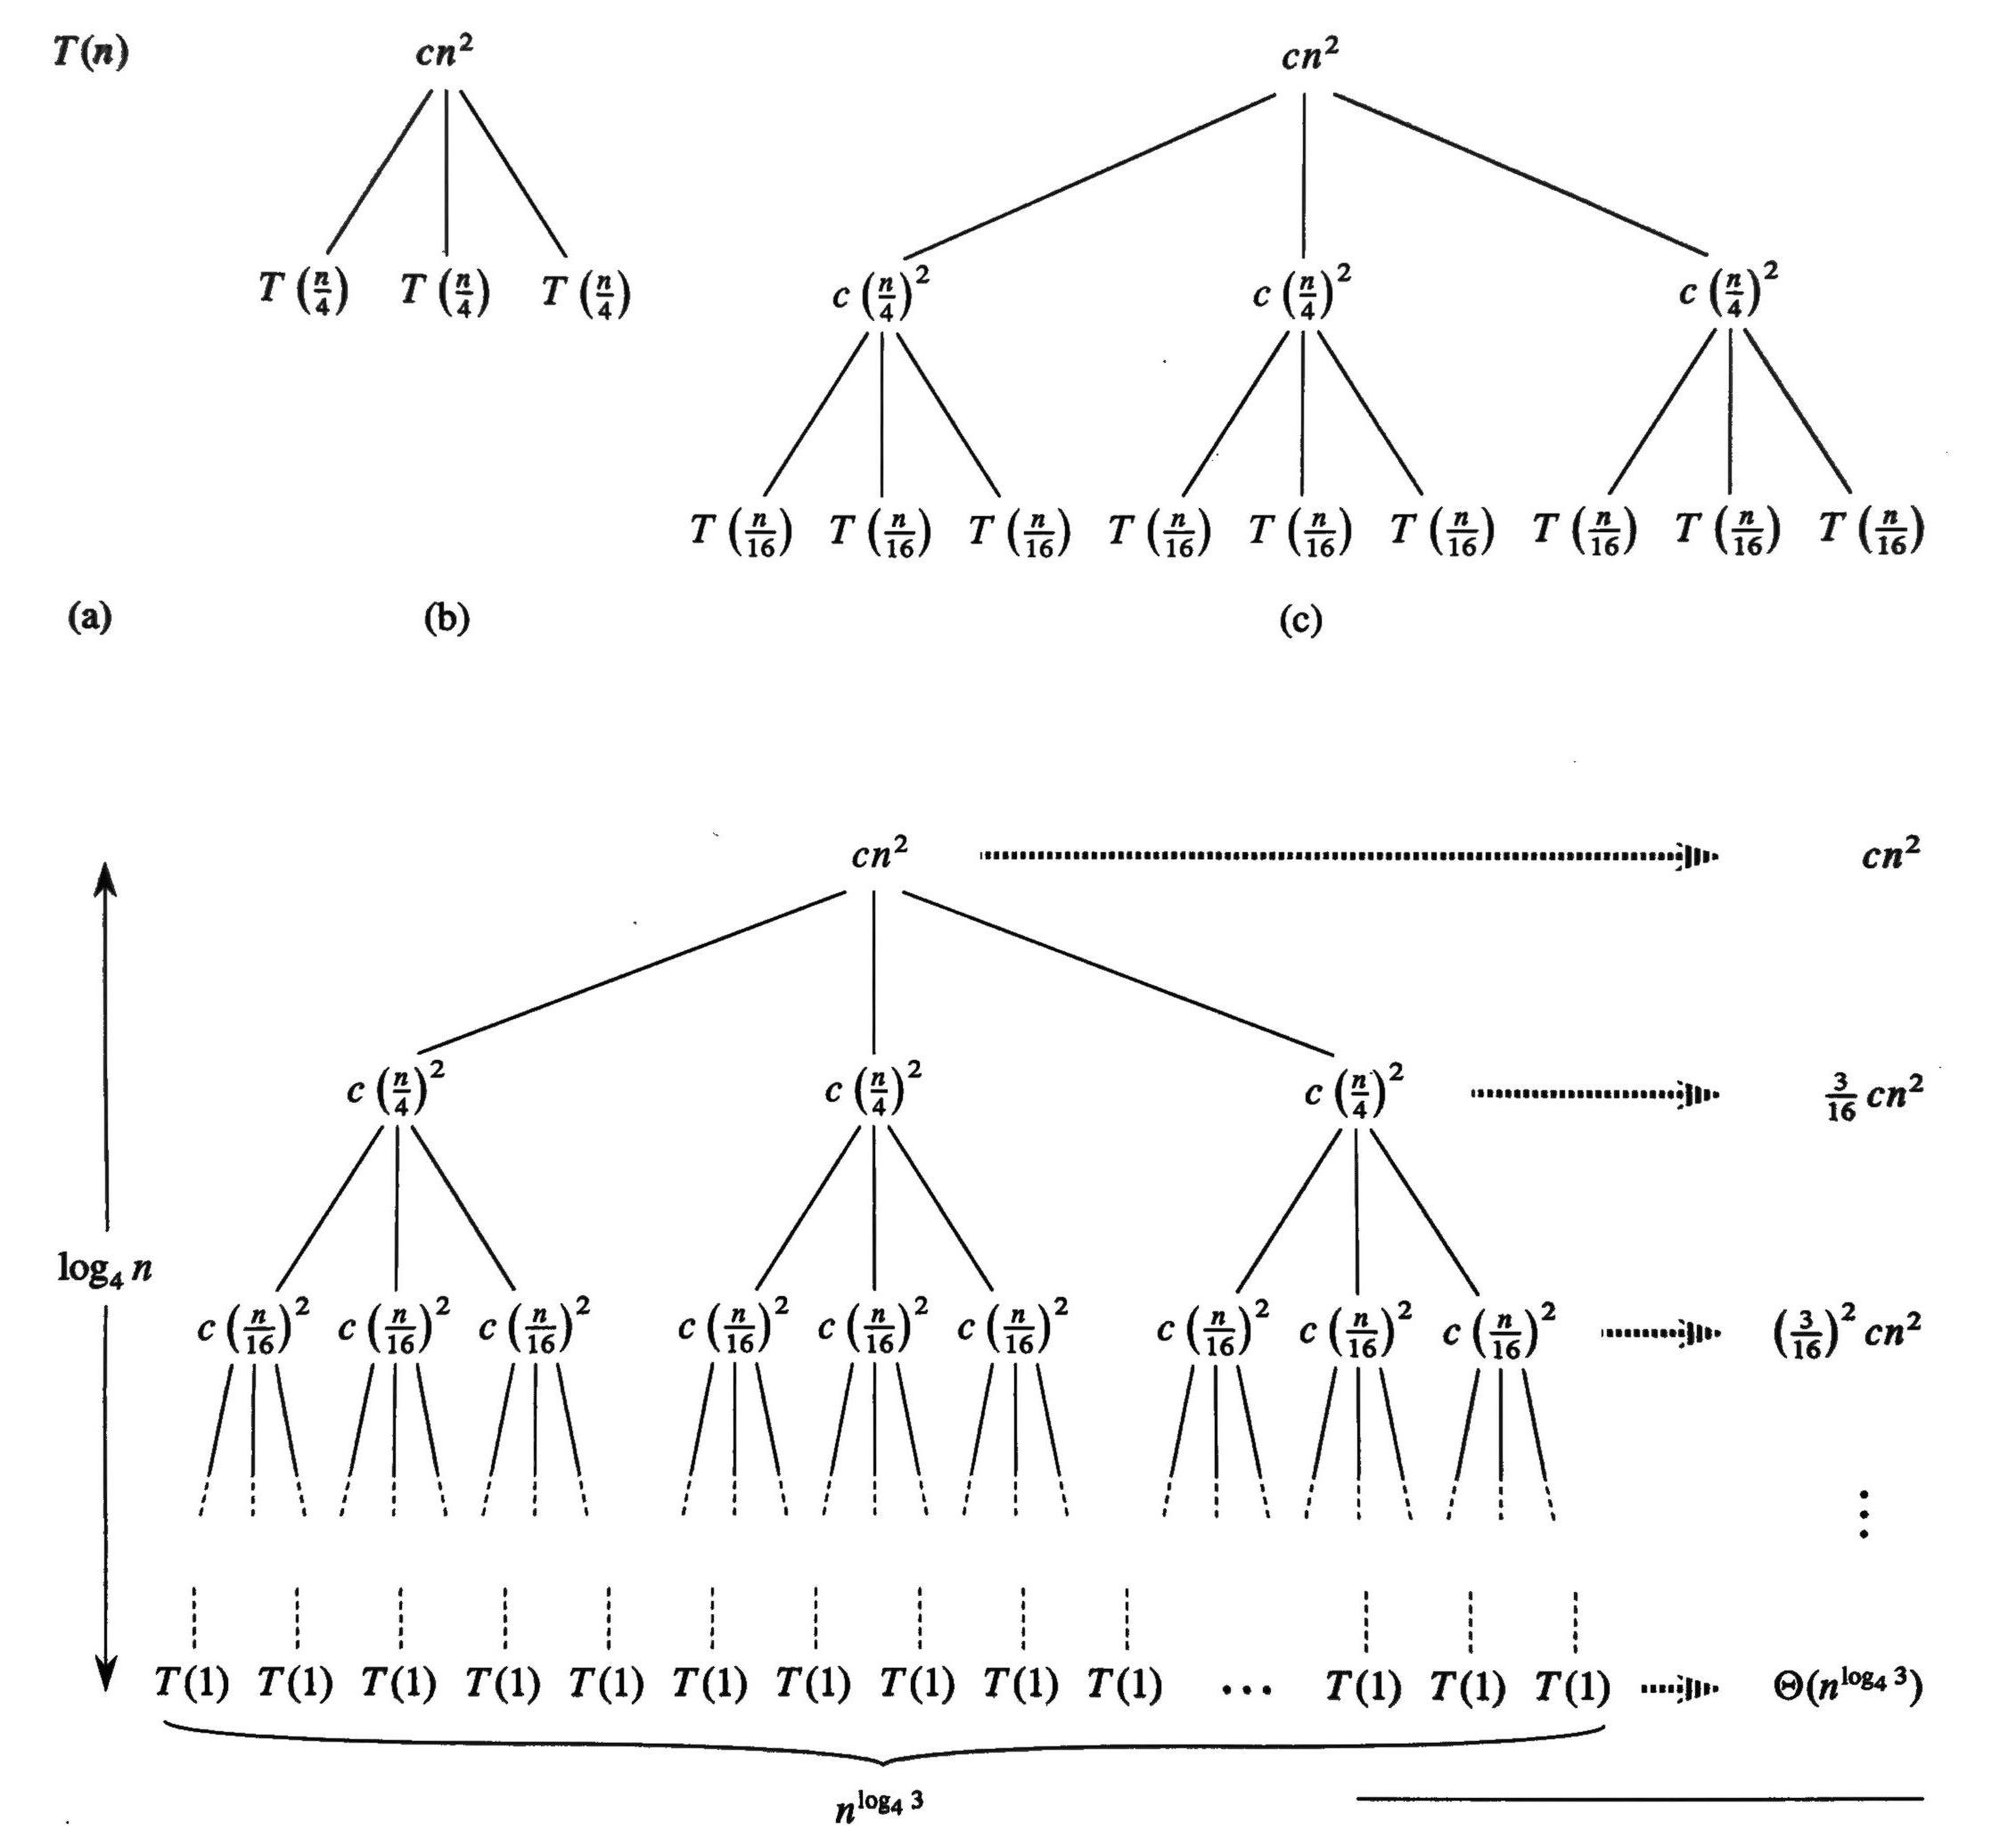
\includegraphics[width=10cm]{albero ricorrenze.jpg}
  \caption{Albero della ricorrenza \(T(n)=3T(n/4)+cn^2\)}
\end{figure}

La parte \((a)\) della figura mostra \(T(n)\), che viene espanso nella parte \((b)\) in un albero equivalente che rappresenta la ricorrenza. Il termine \(cn^2\) nella radice di quest'albero rappresenta il costo al livello più alto della ricorsione, mentre i tre sottoalberi rappresentano i costi richiesti dai tre sottoproblemi di dimensione \(n/4\). La parte \((c)\) mostra l'espansione dei nodi di costo \(T(n/4)\) dalla parte \((b)\), in cui ogni nodo figlio ha costo \(c(n/4)^2\). Tale processo viene ripetuto più e più volte fino ad ottenere i casi base, rappresentati nella parte \((d)\) con \(T(1)\). 

La dimensione dei sottoproblemi per i nodi alla profondità \(i\) è di \(n/4^i\), quindi la dimensione del sottoproblema diventa 1 (dimensione delle foglie) quando \((n/4)^i=1\), ovvero quando \(i=log_4(n)\): dunque, l'albero della ricorrenza ha esattamente \(log_4n+1\) livelli. Ora, per determinare il costo di ogni livello, basti pensare che ogni nodo dell'albero genera tre sottonodi e che, dunque, il numero di nodi alla profondità \(i\) è \(3^i\). Moltiplicando il risultato appena ottenuto con il costo di un singolo nodo, si ottiene che ogni livello ha un costo di \(3^ic(n/4^i)^2 = (3/16)^icn^2\). L'ultimo livello dell'albero conta \(n^{log_43}\) nodi, ognuno di costo \(T(1)\), per un costo totale di \(n^{log_43}T(1)\), ovvero \(\Theta(n^{log_43})\).

A questo punto, si sommano i contributi di ogni livello, ottenendo:
\begin{flalign*}
  T(n)\;\;\; &= \;\;\; cn^2 + \frac{3}{16}cn^2 + \bigg(\frac{3}{16} \bigg)^2cn^2+...+\bigg(\frac{3}{16} \bigg)^{log_4n-1}cn^2+\Theta(n^{log_43}) &&\\
  &=\;\;\; \sum_{i=0}^{log_4n-1}\bigg(\frac{3}{16}\bigg)^icn^2+\Theta(n^{log_43}) &&\\
  &\overset{*}{<} \;\;\; \sum_{i=0}^{\infty}\bigg(\frac{3}{16}\bigg)^icn^2+\Theta(n^{log_43}) &&\\
  &= \;\;\; \frac{1}{1-(3/16)}cn^2 + \Theta(n^{log_43}) &&\\
  &= \;\;\; \frac{16}{13}cn^2 + \Theta(n^{log_43}) &&\\
  &= \;\;\; O(n^2).
\end{flalign*}

Il passaggio segnato con * rappresenta una piccola approssimazione: la \(\sum_{i=0}^{log_4n-1}\big(\frac{3}{16}\big)^icn^2\) ammette come limite superiore \(\sum_{i=0}^{\infty}\big(\frac{3}{16}\big)^icn^2\), che rappresenta una serie geometrica decrescente infinita. In questo modo è possibile proseguire con agilità i calcoli, ottenendo come ipotesi \(T(n)=O(n^2)\), che dovrà essere verificata con il metodo della sostituzione. 

\subsection{Metodo dell'Esperto}
Il metodo dell'esperto è impiegato per la risoluzione di ricorrenze del tipo \(T(n)=aT(n/b)+f(n)\), con \(a\ge 1, b>1\) costanti ed \(f(n)\) una funzione asintoticamante positiva. Una ricorrenza di questo tipo rappresenta il tempo di esecuzione di un algoritmo che divide il problema di dimensione \(n\) in \(a\) sottoproblemi di dimensione \(n/b\), mentre la funzione \(f(n)\) rappresenta il costo di divisione del problema e di combinazione delle soluzioni.
Il metodo dell'esperto dipende dal seguente teorema:

\begin{theorem}[Master Theorem]
  Date le costanti \(a\ge 1\), \(b>1\) e la funzione \(f(n)\), se la ricorsione \(T(n)\) si presenta nella forma \(T(n)=aT(n/b)+f(n)\), allora può essere limitata asintoticamente nei seguenti modi:
  \begin{enumerate}
    \item Se \(f(n)=O(n^{log_b a-\varepsilon})\) per qualche \(\varepsilon>0\), allora \(T(n)=\Theta(n^{log_b a})\);
    \item Se \(f(n)=\Theta(n^{log_b a})\), allora \(T(n)=\Theta(n^{log_b a}log_2(n))\);
    \item Se \(f(n)=\Omega(n^{log_b a +\varepsilon})\) per qualche \(\varepsilon>0\) e se \(af(n/b)\le cf(n)\) per qualche \(c<1\) e per ogni \(n\) sufficientemente grande, allora \(T(n)=\Theta(f(n))\).
  \end{enumerate}
\end{theorem}

Si osservi che in ciascuno dei tre casi, si confronta la funzione \(f(n)\) con la funzione \(n^{log_b a}\): intuitivamente, la soluzione della ricorrenza è determinata dalla funzione polinomialmente \footnote{Una funzione è polinomialmente più grande rispetto ad un'altra funzione se la prima è asintoticamente più grande della seconda di un fattore \(n^\varepsilon\) per qualche \(\varepsilon >0\).} più grande. Se la funzione \(n^{log_b a}\) è più grande polinomialmente, come nel caso uno, allora sarà soluzione della ricorrenza, altrimenti la soluzione sarà \(f(n)\), come enunciato nel caso tre, in cui si deve anche verificare la condizione di regolarità della funzione. Nel caso due, in cui le due funzioni sono asintoticamente uguali, si moltiplicano entrambi i membri per un fattore logaritmico e la soluzione sarà \(T(n)=\Theta(n^{log_b a}log_2(n)) = \Theta(f(n)log_2(n))\).

I tre casi, sfortunatamente, non coprono tutte le funzioni \(f(n)\) possibili, in quanto ci sarà un intervallo fra i casi 1 e 2, in cui la funzione \(f(n)\) è minore di \(n^{log_b a}\), ma non polinomialmente, mentre ci sarà anche un intervallo fra i casi 2 e 3, in cui la funzione \(f(n)\) è maggiore di \(n^{log_b a}\), ma non polinomialmente. In questi casi, il teorema dell'esperto non può essere applicato. 

Per utilizzare il teorema enunciato, bisogna semplicemente determinare in quali dei tre casi rientra la funzione \(f(n)\) e confrontarla con la funzione \(n^{log_b a}\).

\textit{ESEMPIO:} Si determini la soluzione della ricorrenza \(T(n)=9T(n/3)+n\). In questo caso, si ha che \(a=9, b=3\) ed \(f(n)=n\) e quindi \(n^{log_b a} = n^{log_3(9)}=\Theta(n^2)\). Dato che \(f(n)=O(n^{log_3(9)-\varepsilon})\), con \(\varepsilon = 1\) (in quanto \(f(n)=n\)), si può applicare il caso 1 del teorema dell'esperto e concludere immediatamente che la soluzione della ricorrenza è \(T(n)=\Theta(n^2)\), in quanto \(n^2\) è polinomialmente più grande di \(n\). 

\vspace*{10pt}

\textit{ESEMPIO:} Si determini la soluzione della ricorrenza \(T(n)=2T(n/2)+n\,log_2\,n\). In questo caso, si ha che \(a=2,b=2\) ed \(f(n)=n\,log_2\,n\) e quindi \(n^{log_b a}=n^{log_2(2)} = n\). Si potrebbe erroneamente pensare di essere nel terzo caso del teorema dell'esperto, ma le due funzioni non sono polinomialmente comparabili quindi non si può applicare il teorema. La ricorrenza, dunque, deve necessariamente essere risolta con l'utilizzo dei metodi precedentemente analizzati.

\section{Heap Sort}
Analizzando l'algoritmo Merge Sort si è constatato che è efficiente dal punto di vista temporale, ma non dal punto di vista spaziale, in quanto occupa una grande quantità di memoria. A questo proposito, si analizza ora l'algoritmo \textbf{Heap Sort}, che effettua un ordinamento sul posto degli elementi utilizzando una struttura dati detta Heap ('mucchio'), per la gestione delle informazioni.

Un Heap (binario) è una struttura dati ad albero binario quasi completo \footnote{Un albero binario quasi completo è una struttura dati ad albero in cui ogni livello è completo, eccetto per al più l'ultimo livello, che potrebbe essere completo solo fino ad un certo punto da sinistra}, in cui ogni nodo rappresenta un elemento dell'array da ordinare. Nello specifico, \code{A[1]} è la radice dell'albero, e per ogni elemento \code{A[i]}, \code{A[2i]} e \code{A[2i+1]} rappresentano i figli del nodo, mentre \lstinline[mathescape]{A[$\lfloor n/2 \rfloor$]} rappresenta il nodo padre. Si possono quindi definire le seguenti procedure:

\begin{lstlisting}[mathescape=true]
parent(i):
  return $\lfloor i/2 \rfloor$
\end{lstlisting}
\begin{lstlisting}[mathescape=true]
left(i):
  return $2i$
\end{lstlisting}
\begin{lstlisting}[mathescape]
right(i):
  return $2i+1$
\end{lstlisting}

Oltre all'attributo \code{A.length}, che ne ritorna la lunghezza, l'array \code{A} possiede in questo caso anche l'attributo \code{A.heapSize}, che indica il numero degli elementi dell'heap che sono registrati nell'array \code{A}. In altre parole, anche se l'array contiene \(n\) elementi, con \(n\)=\code{A.length}, soltanto gli elementi in \code{A[1..A.heapSize]}, con \(0\le\) \code{A.heapSize} \(\le\) \code{A.length}, sono elementi validi dell'heap.

Esistono, inoltre, due tipologie di heap binari: max-heap e min-heap. Il primo, più importante, è costruito in modo tale che ogni nodo rispetti la condizione per cui \lstinline[mathescape]{A[parent(i)] $\ge$ A[i]}; dunque, il valore di un nodo è al massimo il valore del nodo padre e, di conseguenza, l'elemento più grande di un max-heap è memorizzato alla sua radice. Il secondo, meno utilizzato, è costruito in modo tale che ogni nodo rispetti la condizione per cui \lstinline[mathescape]{A[parent(i)] $\le$ A[i]}. 

Per implementare l'algoritmo heapsort si fa utilizzo del max-heap; per poterne mantenere le proprietà si utilizza la procedura di supporto \code{maxHeapify}, un algoritmo che prende in input un array \code{A} e un suo indice \code{i}, e restituisce l'array ordinato in modo tale da rappresentare il max-heap. Quando tale procedura viene invocata, essa assume che gli alberi binari di radici \code{left(i)} e \code{right(i)} siano dei max-heap, ma assume anche che \code{A[i]} possa essere più piccolo dei suoi figli, violando la proprietà fondamentale. La procedura, quindi, ha il compito di far 'scendere' il valore \code{A[i]} in modo tale che il sottoalbero con radice di indice \(i\) diventi un max-heap.

\vspace{1in}

In pseudocodice:
\lstinputlisting[mathescape]{../docs/algorithms/max_heapify.txt}
 
A ogni passo viene determinato il più grande degli elementi \code{A[i]}, \code{A[left(i)]} e \code{A[right(i)]} e il suo indice viene memorizzato nella variabile \code{max}. Se \code{A[i]} è l'elemento più grande, allora il sottoalbero è già un max-heap e la procedura termina la propria esecuzione, altrimenti uno dei due figli contiene l'elemento più grande e \code{A[i]} viene scambiato con \code{A[max]} (\code{swap with}); in questo modo, il nodo di indice \(i\) e i suoi figli soddisfano la proprietà di max-heap. Il nodo con indice massimo, però, presenta il valore originale di \code{A[i]} e, quindi, il sottoalbero di radice \code{max} potrebbe violare la proprietà fondamentale: quindi, la procedura viene chiamata ricorsivamente sul sottoalbero, fino a raggiungere le foglie.

Questa procedura viene eseguita in un tempo \(O(h)\), con \(h\) l'altezza dell'albero. Essendo l'albero quasi completo, \(h=O(log\,n)\), quindi \(T(n)=O(log\,n)\).

\vspace*{10pt}

Ora, tramite la procedura \code{maxHeapify} è possibile convertire un array \code{A[1..n]} (con \(n\)=\code{A.length}) in un max-heap. Prima di procedere, è importante osservare come tutti gli elementi \lstinline[mathescape]{A[$\lfloor n/2 \rfloor + 1$ .. n]} siano foglie dell'albero e, quindi, ciascuno di essi è un heap di un solo elemento, che si può utilizzare come punto di partenza per la costruzione dell'heap. Si introduce, dunque, la procedura \code{buildMaxHeap}, che attraversa i nodi restanti dell'albero ed esegue la procedura \code{maxHeapify} in ciascuno di essi. 

In pseudocodice:
\lstinputlisting[mathescape]{../docs/algorithms/build_max_heap.txt}

Si può dimostrare che tale procedura impiega un tempo di esecuzione \(T(n)=O(n)\).

\vspace*{10pt}

A questo punto, è possibile scrivere l'algoritmo \code{heapSort}. In pseudocodice:

\lstinputlisting[mathescape]{../docs/algorithms/heap_sort.txt}

Questo algoritmo si basa sul fatto che, una volta riordinato l'array in maniera che rappresenti un max-heap, l'elemento più grande dell'array si trova in \code{A[1]}: questo elemento può quindi essere inserito nella posizione finale corretta scambiandolo con \code{A[n]}. Se ora si toglie il nodo \(n\) dall'heap, diminuendo \code{A.heapSize}, si nota che i figli della radice restano max-heap, ma la nuova radice potrebbe violare la proprietà del max-heap. Questo problema può essere rimosso chiamando la procedura \code{maxHeapify(A, 1)}, che lascia un max-heap in \code{A[1..n-1]}. Questa operazione viene ripetuta fino ad un heap di dimensione 2, già ordinato per definizione. 

Come detto in precedenza, la procedura \code{buildMaxHeap} impiega un tempo di esecuzione lineare (\(O(n)\)), mentre le \(n-1\) chiamate alla procedura \code{maxHeapify} impiegano ciascuna un tempo \(O(log\,n)\). Pertanto il tempo di esecuzione dell'\code{heapSort} impiega un tempo di esecuzione \(T(n)=O(n\,log\,n)\).

\section{Quick Sort}
\textbf{Quick sort} è un algoritmo di ordinamento divide et impera, il cui tempo di esecuzione nel caso peggiore è \(O(n^2)\). Nonostante un tempo di esecuzione molto lento nel caso peggiore, quick sort è uno degli algoritmi più utilizzati perchè ha un tempo medio atteso \(\Theta(n\,log\,)\) e i fattori costanti nascosti dalla notazione asintotica sono pressochè nulli. Inoltre, è un algoritmo di ordinamento sul posto, che lo rende utilizzabile anche in calcolatori con memoria limitata. 

L'idea generale di questo algoritmo si basa sui tre tipici passi del metodo divide et impera, per un sottoarray \code{A[p..r]}:
\begin{enumerate}
  \item Divide: partiziona l'array \code{A[p..r]} in due sottoarray \code{A[p..q-1]} e \code{A[q+1..r]} (eventualmente vuoti) tali che ogni elemento di \code{A[p..q-1]} sia minore o uguale di \code{A[q]} che, a sua volta, è minore o uguale di ogni elemento di \code{A[q+1..r]}.
  \item Impera: ordina i due sottoarray \code{A[p..q-1]} e \code{A[q+1..r]} chiamando ricorsivamente sè stesso.
  \item Combina: nessuna operazione di ricombinazione necessaria in quanto l'array \code{A[p..r]} è già ordinato.
\end{enumerate}

La procedura \code{quickSort} è implementata tramite il seguente pseudocodice:

\lstinputlisting{../docs/algorithms/quick_sort.txt}

Per pter ordinare un intero array \code{A}, la chiamata iniziale a tale algoritmo è \code{quickSort(A, 1, A.length)}. Si noti che all'interno di tale algoritmo viene chiamata la sottoprocedura \code{partition}, definita come segue in pseudocodifica:

\lstinputlisting{../docs/algorithms/partition.txt}

Questo algoritmo riarrangia il sottoarray \code{A[p..r]} sul posto selezionando un elemento \code{x = A[r]} come pivot, intorno a cui partizionare l'array. All'inizio di ogni iterazione del ciclo \code{for} di riga 4, per qualsiasi indice \(k\) si individuano quattro regioni:
\begin{enumerate}
  \item Se \(p\le k\le i\), allora \lstinline[mathescape]{A[k] $\le$ x};
  \item Se \(i+1\le k \le j-1\), allora \lstinline[mathescape]{A[k] $\ge$ x};
  \item Se \(k=r\), allora \code{A[k]=x};
  \item Gli indici \(k\) tali che \(j \le k \le r-1\) non hanno una particolare relazione con il pivot \(x\).
\end{enumerate}

Le ultime due righe della procdeura, inveceinseriscono il pivot al suo posto nel mezzo dell'array, scambiandolo con l'elemento più a sinistra, che è maggiore di \(x\), e restituisce un nuovo indice di pivot. Il tempo di esecuzione dell'algoritmo \code{partition} con input il sottoarray \code{A[p..r]} è \(\Theta(n)\), con \(n=r-p+1\).

Il tempo di esecuzione dell'algoritmo \code{quickSort} dipende solamente da come viene partizionato l'array (in maniera bilanciata o meno) che, a sua volta, dipende da quali elementi vengono utilizzati per il partizionamento. Se il partizionamento è bilanciato, l'algoritmo ha un tempo di esecuzione \(\Theta(n\,log\,n)\), mentre nel caso peggiore, quando il partizionamento è sbilanciato, l'algoritmo converge ad una solzuione in un tempo \(\Theta(n^2)\).

\vspace*{10pt}

Il comportamento nel caso peggiore si verifica quando la subroutine \code{partition} produce un sottoproblema con \(n-1\) elementi e uno vuoto. Per calcolare il tempo di esecuzione, si suppone che questo sbilanciamento si verifichi per ogni chiamata ricorsiva. Il partizionamento costa un tempo di esecuzione \(\Theta(n)\) e, dato che uno dei due array è vuoto e làaltro conta \(n-1\) elementi, si ha un tempo totale:
\begin{equation*}
  T(n) = T(n-1) + T(0) + \Theta(n) = T(n-1) + \Theta(1) + \Theta(n)
\end{equation*}
Intuitivamente, e si sommano i costi ad ogni livello della ricorsione si ottiene una serie aritmetica, il cui valore è \(\Theta(n^2)\). Questa situazione si verifica quando l'array di partenza è già completamente ordinato. 

\vspace*{10pt}

Il comportamento nel caso ottimo si verifica quando la subroutine \code{partition} produce due sottoproblemi di dimensione non maggiore di \(n/2\): in questo caso il tempo di esecuzione dell'algoritmo è molto più rapido e avviene in un tempo totale \(T(n) \le 2T(n/2) + \Theta(n)\), che per il secondo caso del teorema dell'esperto, ha soluzione \(T(n)=\Theta(n\,log\,n)\). Si noti, inoltre, che nel caso in cui la partizione non fosse perfettamente bilanciata, l'algoritmo riuscirebbe comunque a riordinare l'array in un tempo \(T(n)=\Theta(n\,log\,n)\): questo dimostra che il \code{quickSort} è un algoritmo molto più vicino al caso ottimo che al caso pessimo, caso che si verifica in una sola istanza del problema (quando, appunto, è ordinato). 

\vspace*{10pt}

Il comportamento nel caso medio si verifica quando la subroutine \code{partition} produce una combinazione di partizioni 'buone' e 'cattive'. Si suppone, per semplicità, che le partizioni buone e cattive si alternino all'interno dell'albero di ricorsione e che quelle buone siano tutte nel caso migliore, mentre le quelle cattive siano nel caso pessimo. Si ipotizzi che nella radice dell'albero il costo di ripartizione è \(n\) e i sottoarray prodotti hanno dimensione \(n-1\) e 0 (caso pessimo), mentre nel livello successivo il prtizionamento del sottoarray \(n-1\) produca due array di dimensione \((n-1)/2\) e \((n-1)/2 - 1\) (caso migliore). Il costo di una divisione cattiva, seguito da una divisione buona è comunque \(\Theta(n)\), ovvero lo stesso costo di una divisione buona: intuitivamente, quindi, la coppia divisione buona/cattiva impiega lo stesso tempo totale di esecuzione \(\Theta(n\,log\,n)\), con l'unica differenza che cambiano le costanti moltiplicative, eclissante nella notazione asintotica.

\section{Counting Sort}
Gli algoritmi analizzati fino ad ora, seppur differenti fra loro, condividono un'importante proprietà: l'ordinamento che effettuano è basato soltanto su confronti fra gli elementi di input. Questi algoritmi sono detti di ordinamento per confronti e, dati due elementi \(a_i\) e \(a_j\), eseguono uno dei test \(a_i < a_j, a_i\le a_j, a_i=a_j, a_i\ge a_j\) o \(a_i > a_j\) per determinare il loro ordine relativo. 

Gli algoritmi di ordinamento per confronti possono essere visti in termini di alberi di decisione, ovvero alberi binari completi che rappresentano i confronti fra gli elementi effettuati da un determinato algoritmo di ordinamento. Ora, l'esecuzione di un algoritmo di ordinamento corrisponde ad indicare su tale albero un cammino semplice che collega la radice dell'albero con una foglia (nello specifico, una delle foglie che rappresentano le permutazioni ordinate dell'array di ingresso). Ogni nodo interno di tale albero rappresenta un confronto: il sottoalbero sinistro corrisponde a confronti del tipo \(a_i \le a_j\), mentre quello destro corrisponde a confronti del tipo \(a_i > a_j\). Si noti che sulle foglie sono presenti tutte le possibili permutazioni della sequenza di input: dunque un albero di decisione può presentare più di \(n!\) foglie, in quanto alcune permutazioni potrebbero comparire più volte, ma meno di \(2^h\) (con h, l'altezza dell'albero). La lunghezza del cammino semplice più lungo dalla radice di un albero di decisione ad una delle sue foglie rappresenta il numero di confronti che un determinato algoritmo di ordinamento deve svolgere nel caso peggiore: questo numero è equivalente all'altezza dell'albero stesso. Si introduce quindi il seguente teorema, che determina un limite inferiore sul tempo di esecuzione degli algoritmi di ordinamento per confronti:

\begin{theorem}
  Qualsiasi algoritmo di ordinamento per confronti richiede \(\Omega(n\,log\,n)\) confronti nel caso peggiore.
\end{theorem}

\noindent
da cui deriva anche:

\begin{theorem}
  Ogni albero di decisione di un algoritmo di ordinamento di n elementi ha altezza \(\Omega(n\,log\,n)\).
\end{theorem}

\vspace*{10pt}

Una volta determinato il limite inferiore del tempo di esecuzione degli algoritmi di ordinamento, si introduce qui l'algoritmo \textbf{counting sort}, che riordina un array di dimensione \(n\) in un tempo lineare \(\Theta(n)\). 
Tale algoritmo suppone che ciascuno degli elementi di input sia un numero intero compreso nell'intervallo da 0 a \(k\in \mathbb{N}\) e determina per ciascun di essi il numero di elementi minori; utilizza poi questa informazione per inserire l'elemento corrente direttamente nella giusta posizione nell'array di output. Ad esempio, se l'elemento \(x\) è più grande di 5 altri elementi, allora verrà inserito nella posizione 6 dell'array di output.

Nel codice di counting sort, si suppone che l'input sia un array \code{A[1..n]}, con \(n\)=\code{A.length}. Occorrono altri due array: l'array \code{B[1..n]}, che contiene l'output ordinato, e l'array \code{C[0..k]} fornisce la memoria temporanea di lavoro. In pseudocodice:

\lstinputlisting{../docs/algorithms/counting_sort.txt}

Dopo che il ciclo \code{for} in riga 3 inizializza a zero tutti gli elementi dell'array \code{C}, ogni elemento dell'input viene esaminato con il secondo ciclo \code{for} (in riga 5): se il valore di un elemento è \(i\), viene incrementato il valore di \code{C[i]}. Dunque, dopo la riga 6, l'array \code{C} contiene il numero di elementi uguagli ad \(i\), per ogni \(i=0,1,...,k\). Le righe 7 e 8 determinano, per ogni \(i=0,1,...,k\), quanti elementi di input sono minori o uguali a \(i\). Infine, il ciclo \code{for} di riga 9 inserisce l'elemento corrente nella posizione corretta all'interno dell'array di output \code{B}. 

Il primo ciclo \code{for} impiega un tempo di esecuzione \(\Theta(k)\), il secondo un tempo \(\Theta(n)\), il terzo un tempo \(\Theta(k)\) e, infine, il ciclo \code{for} di riga 9 impiega un tempo di esecuzione lineare \(\Theta(n)\). Dunque, il tempo di esecuzione totale dell'algoritmo \code{countingSort} è \(T(n)=\Theta(n+k)\). Di solito, questa procedura viene utilizzata quando \(h=\Theta(n)\), facendo si che il tempo totale di esecuzione sia un \(\Theta(n)\). 

L'algoritmo appena analizzato batte il limite inferiore di tempo \(\Omega(n\,log\,n)\) per gli algoritmi di ordinamento per confronti perchè non confronta nessun elemento dell'input, ma utilizza il valore di ogni elemento come indice di un array \code{C} di appoggio. 




